\subsection{Upplägg}
\label{Upplagg}

\begin{figure}[htb!]\centering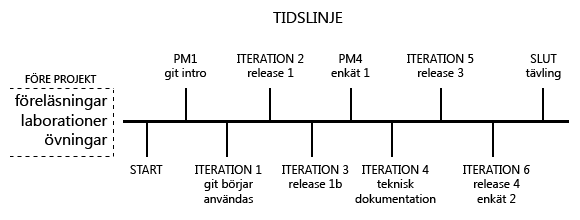
\includegraphics[width=0.75\textwidth]{Tidslinje.png}\caption{Visar tidsupplägget i projektet med viktiga händelser (PM = Planeringsmöte)}\label{fig:Timeline}\end{figure}

Vi lade upp arbete så att vi inte skulle lägga för mycket fokus på att använda Git som VCS då det är mycket ny information. Vårt team som vi skulle utbilda har inte varit i någon kontakt med Git innan men har inte heller några djuprotade arbetssätt med något annat VCS. Vi har delat upp upplägget för gruppen i tre faser. Första fasen är rent teoretisk och vi försöker hålla den på så grundläggande nivå som möjligt. Vi måste ständigt hålla i åtanke att för de flesta i gruppen som vi introducerar Git till har aldrig arbetat med något projekt av denna storlek innan. Detta innebär att de har fullt upp med mycket annat och ger vi dem för mycket teori så kommer den ändå inte befästas. Gruppen har redan en god insikt till vikten av att kunna arbeta parallellt och vill lära sig mer om det. 

Då vi också var nya till Git bara någon månad tidigare, så förstår vi deras situation och har lättare för att skriva ner en kort guide på de mest nödvändigaste kommandona för att kunna arbeta med vårt projekt [Appendix A]. Denna guide delade vi ut på första planeringsmötet så alla kunde komma igång med att klona ner och arbeta med koden på första långlabben. Vi tilldelade även en i gruppen att läsa på mer teori samt att testa lite själv, på så vis har de en VCS expert inom gruppen då det kan kännas lättare att prata med varandra.
 
Fas två uppstod vid första labben och för det flesta var därmed deras mer teoretiska lärande färdigt. Här efter fick de uteslutande lära sig av vad de såg och gjorde. Det vill säga att de såg vilka fördelar Git har och i vilka situationer man bör  använda sig av olika funktioner. I fas två var gruppen fortfarande väldigt outbildad vilket ledde till att vi coacher fick gå  runt och hjälpa dem vid de mer komplicerade kommandon och händelser. Till att börja med så behövde de inte lära sig dessa alls utan bara kunna det som gavs till dem i fas ett. Allt efter som så fick de själva skriva in kommandona och då vi stod bakom och instruerade och endast kontrollerade så att allt gjordes rätt. Vissa i gruppen som inte ville lära sig så mycket om Git stannade i denna fas.

Efter några veckor av labbande anpassade sig  fler och fler i gruppen efter arbetssättet och de tillkallade oss inte då de redan visste vilka kommandon som skulle skrivas. De var då som fas tre inleddes med mycket mer självgående användande utav Git. De visste själva vad som skulle göras och kom själva med förslag när de ville brancha för att till exempel arbeta i tätt samarbete med en annan grupp, t.ex med argument för att uppnå ett bättre resultat snabbare. För sådana strukturella beslut som om det skull gå snabbare att två grupper branchar ut och arbetar tillsammans godkännde vi det först. Detta gjorde vi inte för att de tekniskt skulle ha svårt med det utan att vi ville utvärdera om det skulle finns någon vinning i det.

Det var för det mesta väldigt säkert att låta grupperna själva experimentera så fort de hade lärt sig grunderna eftersom Git är väldigt robust och man kan nästan alltid återskapa ändringarna. Att återskapa ändringar var speciellt endkelt för oss i Git då vi hade minst fem stycken lokala repon med komplett historik samt en server. Då de följer den utdelade guiden och ofta commitar upp till sina egna lokala repon så kan man återställa så gott som allt.

\subsection{Planeringsmöten}

I slutet av varje långlabb fick studenterna skriva ett par meningar om den specifika XP practice som de hade fokuserat på. Vi lade även till att de ska skriva om saker och ting som gick bra och mindre bra med gruppen och vårt arbete, där vi belyste att om det var några problem med Git så skulle de gärna ta upp dem då vi coacher lättare skulle kunna ta tag och åtgärda dem. Dessa punkter togs sedan upp på våra schemalagda planeringsmöten för diskussion och reflektion. Vi kom med förslag till lösningar på hur vi skulle åtgärda dessa och helst så vi attnågon i gruppen hade något sätt. Ett exempel  på en sådan diskussion var om vi behövde skriva en ytterligare guide för att sätta in gruppen i lite svårare funktioner eller om de kunde lära sig dem som beskrivet ovan i \ref{Upplagg} 

I slutet av planeringsmötena delade vi ut spikes till studenterna och om det hade varit något som flera uppfattade som svårt eller problematiskt inom Git så spred vi kunskapen genom att någon fick göra en grundligare undersökning varför det blev så och hur vi skulle kunna göra i fortsättningen. För det absolut mesta så visste vi coacher redan svaret men vi tryckte hårt på att teamet skulle besitta all kunskap själva och inte vara beroende utav oss coacher. Det kunde även förekomma flera tillfällen då gruppen tyckte att det var lättare eller smidigare att fråga varandra istället för oss coacher vilket stödjer att det skulle vara bättre med att gruppen vet allt som de borde. 

Det var viktigt att vi alla i gruppen också skulle kunna ha tillgång till koden hemma för att kunna göra eventuella spikes så som till exempel kod granskning eller undersöka förslag till hur det är bäst att vidareutveckla en viss gren av programmet. För att detta skulle fungera så skrev vi ihop en kort guide på den gemensamma trac-hemsidan. Vi lade också upp ett shell-script som konfigurerar Git till deras inställningar utan att studenterna själva behöver skriva några kommandon.

Under de senare veckorna då gruppen arbetade mer självständigt med Git så skapade vi brancher även för de spikes som kräver något ur repot men även ska uppdatera repot till en ny version när spikesen var klara. Kursledningen hade beslutat att det inte fick skrivas någon kod som trycks upp i repot mellan långlabbarna men gruppen fick till exempel uppdatera JavaDoc eller teknisk dokumentation. Det var viktigt för oss att dessa spikes inte blev för många och att de inte jobbade direkt på vår huvudbranch (master) utan att vi innan långlabben istället kunde merga ihop brancherna. Dessa merges skulle alltid gå automatiskt då det inte skulle vara flera brancher med samma ändringar, även om detta inte alltid var fallet. Till exempel så kunde vi en vecka ha en spike med JavaDoc uppdateringar och en spike med att uppdatera manualen. Dessa två blev således brancher för att kunna arbeta hemifrån utan att störa andra i gruppen som skulle ladda ner koden då de skulle fått en halvt färdig skriven JavaDoc eller manual. Direkt då långlabben startade tog vi en utav brancherna och mergade ihop den med master. Detta blev i Git endast en fast-forward och inga merge konflikter då det bara var en person som hade gjort ändringar. Sedan gick vi till den andra spiken och gjorde det samma. Git löste denna merge-konflikten automatiskt då den tekniska dokumentationen inte hade gjort några ändringar i Java-filer och JavaDocen inte skulle ha gjort några ändringar i den tekniska dokumentationen.

Ledningen för kursen hade även godkänt att större refaktoriseringar utav hela programmets arkitekt kunde vara bra att göra hemma då det för övrigt var produktionsstopp och annars skulle bli väldigt stora och svåra merge konflikter. Då vi hade dessa spikes var det viktigt att den spikegruppen var den enda som arbetade med koden och att alla i gruppen hade en god förståelse på vilka ändringar som skulle göras. Alla i gruppen skulle även veta hur systemet skulle komma att se ut efteråt. Det var viktigt att lägga detta arbete på en egen branch då arbetet kunde göras stegvis med flera commits under tiden. Att göra refaktoriseringar stegvis var inte bara bra för att andra lättare skulle kunna integrera sin kod utan att hela gruppen skulle lättare kunna gå tillbaka om något inte blir bra. En annan mycket viktig aspekt på varför refaktoriseringen inte fick ske på huvudbranchen var om den inte skulle lyckas bli klar så skulle det inte vara några problem och alla kunde bara arbeta på som vanligt. Skulle refaktoriseringen sedan bli klar någon timme in under labben så kan man fortfarande merga ihop den då. Det medför dock att man måste vara noggrann med den funktionalitet som har tillkommit under tiden.

\subsection{Git-konfiguration}

Git är mycket fritt och kan användas på många olika sätt där ingen är bunden att ställa sig i en hierarki. Vi valde dock att arbeta med Git på ett lättförståeligt sätt där alla hämtade(pull) det senaste från en server. På detta vis löste vi det krångliga som kan uppstå med att hämta från flera repon. Alternativet skulle vara att när en grupp har blivit klar med en story så hämtar alla ner hans version och mergar ihop med sitt eget.Det skulle dock bli lite rörigt i vår situation då vi enligt XP anda gjorde parbyten och vilket snabbt slutar med att man inte ha någon aning om vilken dator och inloggning man sitter på. Ett annat vanligt sätt att arbeta på är att ha en så kallad Gatekeeper~\cite{Gatekeeper} som alla hämtar ifrån. När ett par av utvecklare är färdiga med en story så säger man till Gatekeepern som då hämtar från deras, kontrollerar ändringarna och kanske testkör programmet. När han är nöjd säger han till alla att det finns en ny version hos honom som alla ska hämta. Detta sätt är för visso mer säkert och röd kod sprider sig inte när någon har gjort fel. Dock så tyckte vi coacher att detta inte känns så agilt och den snabbheten som är så viktig går lite förlorad. Det skulle även betyda att teamet skulle vara beroende av denna enda “bättre vetande” personen som skulle granska alla arbeten, vilket vi inte heller tyckte går enligt XP. Vi ville med vår grupp uppnå en väldigt självgående sammansättning där vi coacher inte skulle ha någon avgörande roll, och vi vill även att gruppen skulle fungera vi eventuella bortfall. 
Vi valde därför det upplägget som vi gjorde och delade istället ut en task på att något annat utvecklingspar granskar en story innan den anses helt färdig. 


\subsection{Enkätundersökning}

För att mer konkret kunna analysera vår utveckling och ge oss feedback om hur bra materialet och vår undervisning är så har vi lämnat ut en enkät [Appendix B]. I enkäten adresserade vi de olika faserna och se hur framgångsrika de har varit. Vi har ställt enkla frågor för att se hur lätt det var att ta till sig teorin i fas ett och att komma igång med ett naturligt arbetsflöde i fas två. Vi undersökte huruvida de känner sig bekväma med Git och får djupare förståelse för det genom terminalen i steg tre, samt huruvida de skulle kunna tänka sig att arbeta med det i framtiden för en eventuellt fas fyra. Vi gav ut enkäten två gånger under kursens gång för att kunna analysera några förändringar. Den första gången efter cirka halva tiden då de flesta i gruppen var i mitten eller slutet av fas två och den andra gången vi undersöker var på sista mötet då allt arbete med Git var avklarat.
